\chapter{Введение в квантовую механику}

\section{Волна де Бройля}

Альберт Эйнштейн (1905 г.) --- связь корпускулярных $(E, \vp)$ и волновых $(\omega, \vec{k})$ свойств света:

\begin{equation}
\label{eq:1_1_1}
\begin{gathered}
E = \hbar \omega \\ 
\vp = \hbar \vec{k}
\end{gathered}
\end{equation}

$\hbar = 1{,}05 \cdot 10^{-27}$ эрг·с --- постоянная Планка (1900 г.)

Луи де Бройль (1923 г.) --- обобщение волновой теории на материальные частицы (волны вещества). Длина волны де Бройля:

\begin{equation}
\label{eq:1_1_2}
\lambda = \frac{2\pi}{k} = \frac{2\pi \hbar}{p} = \frac{h}{mv}
\end{equation}

\begin{equation}
\label{eq:1_1_3}
\Psi (\vr, t) = A e^{i(\vec{k}\vr - \omega t)}
\end{equation}

Подставляя \eqref{eq:1_1_1} в \eqref{eq:1_1_3}, получим:

\begin{equation}
\label{eq:1_1_4}
\boxed{\Psi(\vr,t) = A e^{\frac{i}{\hbar}(\vp\vr - Et)}}
\end{equation}

\begin{sloppypar}
  \section{Волновой пакет. Фазовая и групповая скорость волн, соответствующих свободной частице}
\end{sloppypar}

Свободная частица характеризуется энергией $E$ и импульсом $\vp~ \|~ Ox$. Волна де Бройля для одномерного случая:

\begin{equation}
\label{eq:1_2_1}
\Psi(x,t) = A e^{\frac{i}{\hbar}(px - Et)}
\end{equation}

Выделим в пространстве поверхность постоянной фазы:

$$\alpha = k x - \omega t = \frac{1}{\hbar} (px - Et) = \const$$

Тогда фазовая скорость запишется в виде:
\begin{equation}
\label{eq:1_2_2}
v_{\text{ф}} = \frac{dx}{dt} = \frac{w}{k} = \frac{E}{p}
\end{equation}

Сравним её с действительной скоростью частицы в двух случаях:

\begin{itemize}
\item Нерелятивистский случай: $E = p^2/{2m}$:  $$v_{\text{ф}} = \frac{p}{2m} = \frac{v}{2}$$
\item  Релятивистский случай: $E = \sqrt{p^2c^2 + m^2c^4}$: $$p = \frac{E}{c^2}v~~\rightarrow~~v_{\text{ф}} = \frac{E}{p} = \frac{c^2}{v} > c$$
\end{itemize}

Таким образом, плоская монохроматическая волна \underline{принципиально} не может описывать свободную частицу. Для этого необходимо использовать волновое образование с \underline{пространственной локализацией}.

Волновой пакет:

\begin{equation}
\label{eq:1_2_3}
\Psi(x,t) = \int^{k_0 + \Delta k}_{k_0 - \Delta k} A(k)e^{i(\vec{k}\vr - \omega (k) t)} dk, \; \Delta k\ll k_0
\end{equation}

\begin{equation}
\label{eq:1_2_4}
\omega (k) = \omega (k_0) + \left. \left ( \frac{d \omega}{dk} \right ) \right |_{k_0} (k-k_0) + \ldots \approx \omega_o +  \left. \left ( \frac{d \omega}{dk} \right ) \right |_{k_0} (k-k_0)
\end{equation}

Подставляя \eqref{eq:1_2_4} в \eqref{eq:1_2_3}:

\begin{equation}
\label{eq:1_2_5}
\psi(x,t) \approx e^{i(k_0 x - \omega_0 t) }\int^{k_0 + \Delta k}_{k_0 - \Delta k} dk A(k)e^{i(k - k_0) \left [ x - \left . \left ( \frac{d\omega}{dk} \right ) \right |_{k_0} t \right ]}
\end{equation}
--- плоская волна с амплитудой, зависящей от координаты и времени.

Постоянство амплитуды волнового пакета:
\begin{equation}
\label{eq:1_2_6}
x - \left . \left ( \frac{d\omega}{dk} \right ) \right |_{k_0} t = const
\end{equation}

Групповая скорость:

\begin{equation}
\label{eq:1_2_7}
v_{\text{гр}} = \frac{dx}{dt} = \left . \left ( \frac{d\omega}{dk} \right ) \right |_{k_0} = \left . \left ( \frac{dE}{dp} \right ) \right |_{p_0}
\end{equation}

Сравним её с действительной скоростью частицы в двух случаях:

$\bullet$ Нерелятивистский случай: $E = p^2/{2m}$:
$$v_{\text{гр}} = \frac{p_0}{m} = v$$

$\bullet$ Релятивистский случай $E = \sqrt{p^2c^2 + m^2c^4}$
$$v_{\text{гр}} = \frac{c^2 2p}{2E} = \frac{c^2 \frac{E}{c^2}v}{E} = v$$

Таким образом, групповая скорость движения пакета как целого, совпадает со скоростью отвечающей ему частицы. 

Обозначим: $\xi = k - k_0$.

$A(k) \approx A(k_0)$ --- пусть амплитуда является слабоменяющейся функцией от $k$.

Подставляя \eqref{eq:1_2_7} в \eqref{eq:1_2_5}, получим:

$$\Psi(x,t) \approx A(k_0) e^{i(k_0 x - \omega_0 t) }\int^{+ \Delta k}_{ - \Delta k} e^{i(x - v_{\text{гр}}t)\xi} d\xi$$

Окончательно:

\begin{equation}
\label{eq:1_2_8}
\Psi(x,t) = 2 A(k_0) \frac{\sin [(x - v_{\text{гр}}t)\Delta k]}{x - v_{\text{гр}}t}e^{i(k_0 x - \omega_0 t)}
\end{equation}

Обозначим:
$$B(x - v_{\text{гр}}t) =  2 A(k_0) \frac{\sin [(x - v_{\text{гр}}t)\Delta k]}{x - v_{\text{гр}}t}$$ --- огибающая волнового пакета, движущаяся с групповой скоростью.

$B(x - v_{\text{гр}}t)$ максимальна, если $x = v_{\text{гр}}t$.

\begin{figure}[h]
\centering
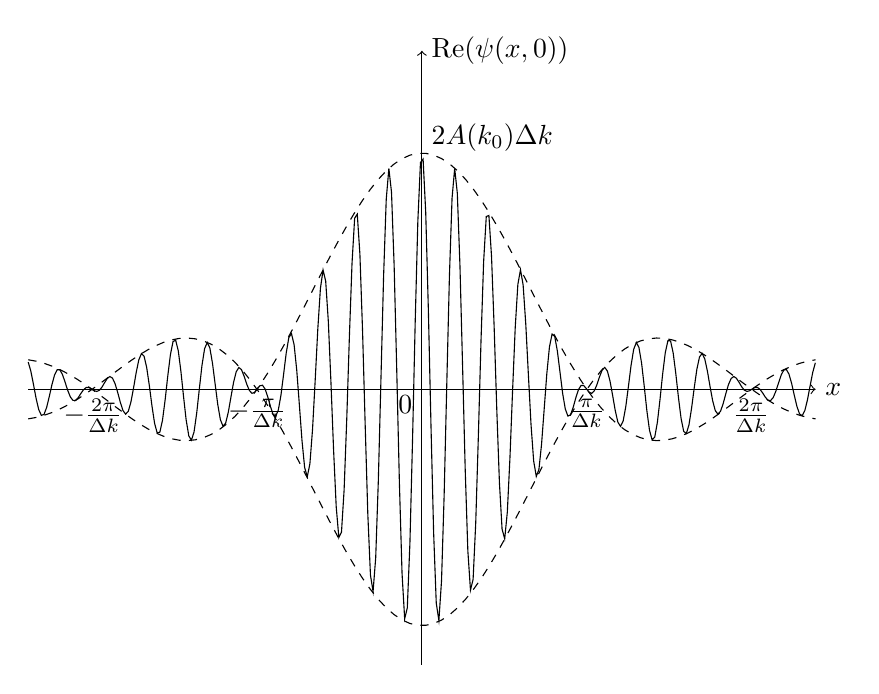
\begin{tikzpicture}[domain=-5:5]
  \draw[->] (-5,0) -- (5,0) node[right] {$x$};
  \draw[->] (0,-3.5) -- (0,4.3) node [right] {Re$(\psi(x, 0))$};
	\draw [dashed, domain=-5:5, samples=100] plot (\x, {2*sin(1.5*\x r) / \x});
  \draw [dashed, domain=-5:5, samples=100] plot (\x, {-2*sin(1.5*\x r) / \x});
  \draw [domain=-5:5, samples=300] plot (\x, {2*sin(1.5*\x r)*cos(15*\x r) / \x});
  \node [left] at (0, -0.2) {$0$};
  \node [below] at (2.09, 0) {$\frac{\pi}{\Delta k}$};
  \node [below] at (-2.09, 0) {$-\frac{\pi}{\Delta k}$};
  \node [below] at (4.18, 0) {$\frac{2\pi}{\Delta k}$};
  \node [below] at (-4.18, 0) {$-\frac{2\pi}{\Delta k}$};
  \node [right] at (0, 3.2) {$2A(k_0) \Delta k$};
\end{tikzpicture}
\caption{Форма волнового пакета при $t=0$.} \label{fig:1_1}
\end{figure}

$$k_0 \gg \Delta k$$

Длина волны много раз укладывается на длине локализации:
$$\lambda = \frac{2 \pi}{k_0} \ll \frac{2 \pi}{\Delta k} = \Delta x$$

\begin{equation}
\label{eq:1_2_9}
\Delta x \cdot \Delta k \approx 1
\end{equation}

Cоотношение неопределенностей Гейзенберга
\begin{equation}
\label{eq:1_2_10}
\boxed{\Delta x \cdot \Delta p \approx \hbar}
\end{equation}

Понятие траектории частицы теряет смысл в квантовой механике!

\begin{sloppypar}
  \section{Уравнение Шрёдингера. Оператор Гамильтона. Общее решение уравнения Шрёдингера в случае, когда гамильтониан не зависит от времени.}
\end{sloppypar}

\textbf{Уравнение Шрёдингера} --- постулат квантовой механики, описывающий эволюцию волновой функции.

Временное (нестационарное) уравнение Шрёдингера:
\begin{equation}
\label{eq:1_3_1}
\boxed{i \hbar \pd{}{t} \Psi(\vr,t) = \left\{ -\frac{\hbar^2}{2m}\vec{\nabla}^2 + U(\vr,t) \right\} \Psi(\vr,t)} 
\end{equation}

Оператор Гамильтона (гамильтониан, оператор полной энергии):
\begin{equation}
\label{eq:1_3_2}
\widehat{H} = \frac{\hat{\vp}^2}{2m} + U(\vr,t)
\end{equation}

Рассмотрим случай, когда потенциальная энергия не зависит от времени:

$$\pd{\widehat{H}}{t} = \pd{U}{t} = 0 $$

Тогда:
\begin{equation}
\label{eq:1_3_3}
\Psi(\vr,t) = \psi(\vr) \cdot \phi (t)
\end{equation}

Подставим \eqref{eq:1_3_3} в уравнение Шрёдингера:

$$i \hbar \psi(\vr) \pd{}{t} \phi (t) = \phi (t) \widehat{H} \psi(\vr)$$

Поделим на $\psi(\vr)\phi(t)$:

$$i \hbar \frac{\partial \phi / \partial t}{\phi(t)} = \frac{\widehat{H} \psi(\vr)}{\psi(\vr)} = E$$

\begin{equation}
\label{eq:1_3_4}
i \hbar \pd{\phi}{t} = E \phi(t)
\end{equation}

\begin{equation}
\label{eq:1_3_5}
i \hbar \pd{}{t} \phi(t) = E \phi(t)
\end{equation}

Стационарное уравнение Шрёдингера:
\begin{equation}
\label{eq:1_3_6}
\boxed{\widehat{H} \psi(\vr) \equiv \left\{ -\frac{\hbar^2}{2m} \vec{\nabla}^2 + U(\vr) \right\}\psi(\vr) = E\psi(\vr)}
\end{equation}

$$\phi(t)=C e^{-\frac{i}{\hbar}Et},$$
где $~C=\phi(0)$

Решение уравнения Шрёдингера представляет собой задачу Штурма-Лиувилля на пары собственных значений и собственных функций: $\{E_k, \psi_k(\vr)\}$, где $k=0,1,2...$

\textbf{Стационарное состояние} --- состояние с определённой энергией.

\begin{sloppypar}
  \section{Статистическая интерпретация волновой функции. Стационарные состояния}
\end{sloppypar}

1926 г., Макс Борн: 

\begin{defn}
Вероятность нахождения частицы в момент времени $t$ в элементе объёма $dv$ в окрестности точки $\vr$:
\begin{equation}
\label{eq:1_4_1}
dP = \Psi^*(\vr,t) \Psi(\vr,t) dv \equiv|\Psi(\vr,t)|^2dv
\end{equation}
\end{defn}

\begin{defn}
Плотность вероятности обнаружения частицы в точке $\vr$ в момент времени $t$:
\begin{equation}
\label{eq:1_4_2}
|\Psi(\vr,t)|^2 = \frac{dP}{dv} = \rho(\vr,t)
\end{equation}
$\Psi(\vr,t)$ --- амплитуда плотности вероятности (амплитуда вероятности)
\end{defn}



Из \eqref{eq:1_4_1} следует условие нормировки волновой функции:

\begin{equation}
\label{eq:1_4_3}
\int |\Psi(\vr,t)|^2 dv = 1
\end{equation}

Таким образом, волновая функция должна быть квадратично интегрируемой.

\begin{exmpl}
Волновой пакет \eqref{eq:1_2_3} подчиняется условию нормировки.
\end{exmpl}

\begin{exmpl}
Волна де Бройля \eqref{eq:1_1_4}:
$$\int |\Psi_{\vp}(\vr,t)|^2 dv = |A|^2 \int dv$$
расходится, поскольку интегрирование проводится по всему пространству
\end{exmpl}


\begin{excr}
Считая, что $\Psi(\vr,t)$ удовлетворяет волновому уравнению \eqref{eq:1_3_1}, доказать:
$$\pd{}{t} \int \rho(\vr,t) dv = 0$$
\end{excr}

\subsection*{Свойства волновой функции}

\begin{enumerate}
\item однозначность
\item конечность
\item \textit{как правило (исключение: задача 4 из 1-го задания)}, непрерывная дифференцируемость $\Psi(\vr,t) \in C^1(\Omega)$
\end{enumerate}

Эти же свойства справедливы и для $|\Psi(\vr,t)|^2$.

\subsection*{Анализ стационарного уравнения Шрёдингера}

\begin{itemize}
\item $\psi(\vr)$ также удовлетворяет вышеперечисленным свойствам волновой функции
\item Нормированность: 
\begin{equation}
\label{eq:1_4_4}
||\psi|| = \int |\psi(\vr)|^2 dv = 1
\end{equation}
\item Граничные условия: $\psi(\vr)|_{r \to \infty} = 0$
\end{itemize}

Временной множитель: $|\phi (t)|^2= |C|^2$.

Из \eqref{eq:1_4_3} и \eqref{eq:1_4_4}: $|C|^2 = 1$, для удобства выберем $C = 1$.

Таким образом, в квантовой механике волновая функция определена с точностью до постоянного фазового множителя.

\subsection*{Общий вид волновой функции стационарного состояния}


$$\boxed{\Psi_E(\vr,t) = e^{-\frac{i}{\hbar}Et} \psi_E(\vr)},$$

где $\widehat{H} \psi_E(\vr) = E\psi_E(\vr)$.

Стоит заметить, что волновая функция зависит от времени (через фазовый множитель).

Общий вид $\Psi(\vr,t)$ для стационарной системы следует рассматривать как синтез волновых, корпускулярных и статистических представлений о микрообъектах. 

Статистическая интерпретация волновой функции относится в том числе и к отдельно взятой частице (1949 г. — экспериментальное доказательство, советские физики Биберман, Сушкин, Фабрикант).

